%\begin{abstract}
%We consider a matched subspace detection problem where a signal vector residing in an unknown low-rank $k$ subspace is to be detected using a subspace estimate obtained from noisy signal-bearing training data with missing entries. The resulting subspace estimate is inaccurate due to limited training data, missing entries, and additive noise. Recent results from random matrix theory (RMT) precisely quantify these subspace estimation errors for the setting where the signal has low coherence. We analytically quantify the ROC performance of the resulting plug-in detector and derive a new detector which explicitly accounts for these subspace estimation errors. The realized increase in performance can be attributed to the new detector only using the $k_\text{eff}\leq k$ ``informative'' signal subspace components. The fraction of observed entries determines $k_\text{eff}$ via a simple relationship that we describe. Detection performance better than random guessing is only achievable when the percent of observed data is above a critical threshold which we explicitly characterize.
%\end{abstract}
%

%\section{Introduction}\label{sec:intro}

%The matched subspace detector (MSD) is a widely used tool in signal processing and machine learning to detect a signal embedded in a low-rank subspace in the presence of additive noise \cite{scharf1994matched,jin2005cfar,mcwhorter2003matched}. The performance of the MSD has been explored when the low-rank signal subspace is known. Scharf and Friedlander \cite{scharf1994matched} consider the MSD when the signal is placed deterministically at an unknown location in a known subspace while McWhorter and Scharf \cite{mcwhorter2003matched} extend this work to allow the signal to be placed randomly with a known (or assumed) distribution in the known subspace.

%There is little work characterizing the performance of the matched subspace detector when the signal subspace is unknown and estimated from data. Recently, we used RMT to quantify the performance of stochastic MSDs in such a setting  \cite{asendorf2011msd}. That work brought into sharp focus the importance of using $k_\text{eff}\leq k$ informative signal subspace components in detector statistics; here $k_{\text{eff}}$ is the effective number of informative components identifiable from limited, noisy data as described in \cite{nadakuditi2008sample}. In this paper, we extend the analysis to the deterministic MSD setting where the training data is noisy \textit{and} has missing entries. The missing entry context is motivated in \cite{balzano2010high} by distributed detection scenarios where it might be prohibitive to collect and transmit only a (randomly chosen) fraction $p$ of the training data entries. Alternately one might think of $1-p \in (0,1)$ as a compression factor as in compressed sensing.

%The main contribution of this paper is a precise quantification of the resulting performance of the MSD. We uncover a phase transition phenomenon by showing that there is a critical fraction, $p_\text{crit}$, which is a simple function of the eigen-SNR, the number of training samples, and the number of sensors, below which detection performance deteriorates to random guessing. Compressing the training dataset below this critical fraction is undesirable.

%The paper is organized as follows. Section \ref{sec:prob stat} formally states the detection problem. Section \ref{sec:rmt} presents pertinent results from RMT. These results are used in Section \ref{sec:derive} to derive a plug-in and random matrix theory MSD and in Section \ref{sec:roc} to derive theoretical ROC curves for each detector. Section \ref{sec:results} validates our analytical predictions, highlights the importance of selecting $k_\text{eff}$ over $k$ subspace components, and demonstrates the effect of missing data. Section \ref{sec:conclusion} presents concluding remarks.

\section{Deterministic Matched Subspace Detectors with Missing Data}\label{sec:chpt3:missing}

We consider the same detection setting as described in Section \ref{sec:msd} using the training
data model in (\ref{eq:taes_train}). However, we only observe a
fraction $p\in(0,1)$ of the entries of our training matrix $Y=[y_1,\dots,y_m]$; $p$ is
independent of $n$ and $m$. Define our observed training data matrix, $\widetilde{Y}$, as
\beq\label{eq:data_model_miss}
\widetilde{Y} = Y\odot M
\eeq
where
\be
 M_{ij} = \begin{cases} 1 & \text{ with probability } \gamma_y\\ 0 & \text{ with
    probability } 1-\gamma_y \end{cases}
\ee
and $\odot$ denotes the Hadamard or element-wise product. Finally we make the following
assumption about our signal subspace, $U$.

\begin{Assum}\label{assum:msd_coher}
In the missing data setting, assume that the columns of $U$ satisfy a `low-coherence'
condition in the following sense: we suppose that there exist 
non-negative constants $\eta$, $C$ independent of $n$, such that for $i=1,\dots,k$ 
\be
\max_i \|u_i\|_\infty \leq \eta\frac{\log^{C}n}{\sqrt{n}}.
\ee
\end{Assum}
We form a signal subspace estimate as in (\ref{eq:param_estims_stoch}), except that we use
our partially observed training matrix $\widetilde{Y}$ to form the sample covariance
matrix $S$ . Call this signal subspace estimate $\widetilde{U}$. 

\subsection{Pertinent Results from RMT}\label{sec:rmt}

By modifying an argument in  \cite{benaych2011singular}, we obtain the following result.
\begin{Th}\label{th:angles}
Assume that $x_i \sim \mathcal{CN}(0,\Sigma^2)$ as in (\ref{eq:taes_train}) and that $U$
in (\ref{eq:taes_train}) obeys the low coherence condition in Assumption
\ref{assum:msd_coher}. Then as $n,m \to \infty$ with $n/m \to c$ we have that
for $i,j = 1, \ldots, k$: 
\begin{equation*}
\begin{aligned}
&|\langle u_i,\widehat{u}_i\rangle|^2\convas
\begin{cases}
1-\dfrac{c\left(1+p\sigma_i^2\right)}{p\sigma_i^2\left(p\sigma_i^2 + c\right)} & \text{ if } \sigma_{i}>\dfrac{c^{1/4}}{\sqrt{p}}\\
0 & \textrm{otherwise}\\
\end{cases}\\
&|\langle u_i,\widehat{u}_j\rangle|^2\convas 0 \qquad \textrm{ for } i \neq j.\\
\end{aligned}.
\end{equation*}
where $\widehat{u}_i$ are the left singular vectors of $\widetilde{Y}$.
\end{Th}

The low coherence condition appears in, for example, \cite{balzano2010high} with the idea
being that the matrix $U \begin{bmatrix} x_{1} & \ldots & x_{m} \end{bmatrix}$ has entries
of about the same magnitude. With the Gaussianity assumption for $x$, all we need is $U$
to have low coherence. Recall that the coherence of a matrix with orthonormal columns is
$\max_{i,j}|U_{i,j}|$. When a matrix is spiky, random sampling of its entries may result
in a loss of information; matrices with low coherence behave better under random sampling
and it is this setting that we focus on in this chapter.

The key insight from Theorem \ref{th:angles} is that only the singular vectors
corresponding to signal singular values above the phase transition
$\frac{c^{1/4}}{\sqrt{p}}$ are \textit{informative}. The fraction of missing entries $p$
regulates this phase transition point as $O(1/\sqrt{p})$. When a signal singular value
drops below this critical threshold, the corresponding singular vector estimate is
essentially noise-like (i.e. $|\langle u_i,\widehat{u}_i\rangle|^2=o_{p}(1)$) and thus
\textit{uninformative}. The term $|\langle u_i,\widehat{u}_i\rangle|^2$ quantifies
mismatch between the estimated and underlying singular vectors; when $p < p_{\text{crit.}}
:=\sqrt{c}/\max_{i}(\sigma_{i}^{2})$ then \textit{all} singular vectors are
uninformative. Intuitively we expect a degradation in the performance of detectors that
utilize subspace components for which $|\langle u_i,\widehat{u}_i\rangle|^2=o_{p}(1)$.  We
refer to the estimate in Theorem \ref{th:angles} as $|\langle
u_i,\widehat{u}_i\rangle|^2_{\text{rmt}}$.

\subsection{Plug-in and RMT Detectors}\label{se:miss_detects}

Using the estimate of our signal subspace, $\widetilde{U}$, formed from our partially
observed training data matrix $\widetilde{Y}$, we define 
\be
\widetilde{w} = \widetilde{U}^Ty
\ee
where $y$ is a testing vector from (\ref{eq:determ_setup}). Note that in this setup, we
don't assume that our testing observation has any missing entries. Following a similar
derivation from Chapter 2 and the previous section, we have our plug-in and RMT test
statistics are
\begin{equation}\label{eq:plugin missing}
\Lambda_{\text{plugin}}(\widetilde{w}) =\widetilde{w}^H\widetilde{w}\sum_{i=1}^k\widetilde{w}_i^2
\end{equation}
\begin{equation}\label{eq:rmt_missing}
\Lambda_{\text{plugin}}(\widetilde{w}) =\widetilde{w}^H\widetilde{w}\sum_{i=1}^{\keff}\widetilde{w}_i^2
\end{equation}
where we define $k_\text{eff}$ as the number of signal singular values above the phase
transition $\frac{c^{1/4}}{\sqrt{p}}$ shown in Theorem \ref{th:angles}. We may use either
test statistic to form a detector of the form 
\begin{equation}\label{eq:opt classifier}
\Lambda(\widetilde{w}) \detgtrless \ln(\eta)
\end{equation}
where $\eta$ satisfies $P(\Lambda(\widetilde{w})>\ln\left(\eta\right)|H_0)=\alpha$.

\subsection{Theoretical ROC Curve Derivation}\label{sec:roc_missing}
A standard way to compare the plug-in and RMT detectors derived in (\ref{eq:plugin missing}) and (\ref{eq:rmt_missing}) respectively is to compute their ROC curves. For a particular statistic $\Lambda(\widetilde{w})$, to compute theoretical ROC curves, we must compute
\begin{equation}\label{eq:target cdf}
\begin{aligned}
&P_D = P(\Lambda(w) > \gamma| w\in H_1)\\
&P_F = P(\Lambda(w) > \gamma| w\in H_0)\\
\end{aligned}
\end{equation}
for $-\infty<\gamma<\infty$. To do this, we explore the conditional CDF under each hypothesis for the statistics (\ref{eq:plugin missing}) and (\ref{eq:rmt_missing}).

This derivation is the same as in Chapter 2 except that we replace $|\langle
u_i,\widehat{u}_i\rangle|_{\text{rmt}}^2$ with the expression in Theorem \ref{th:angles}. 

\section{Simulation Results and Discussion}\label{sec:results}

\begin{figure}[t]
\centering
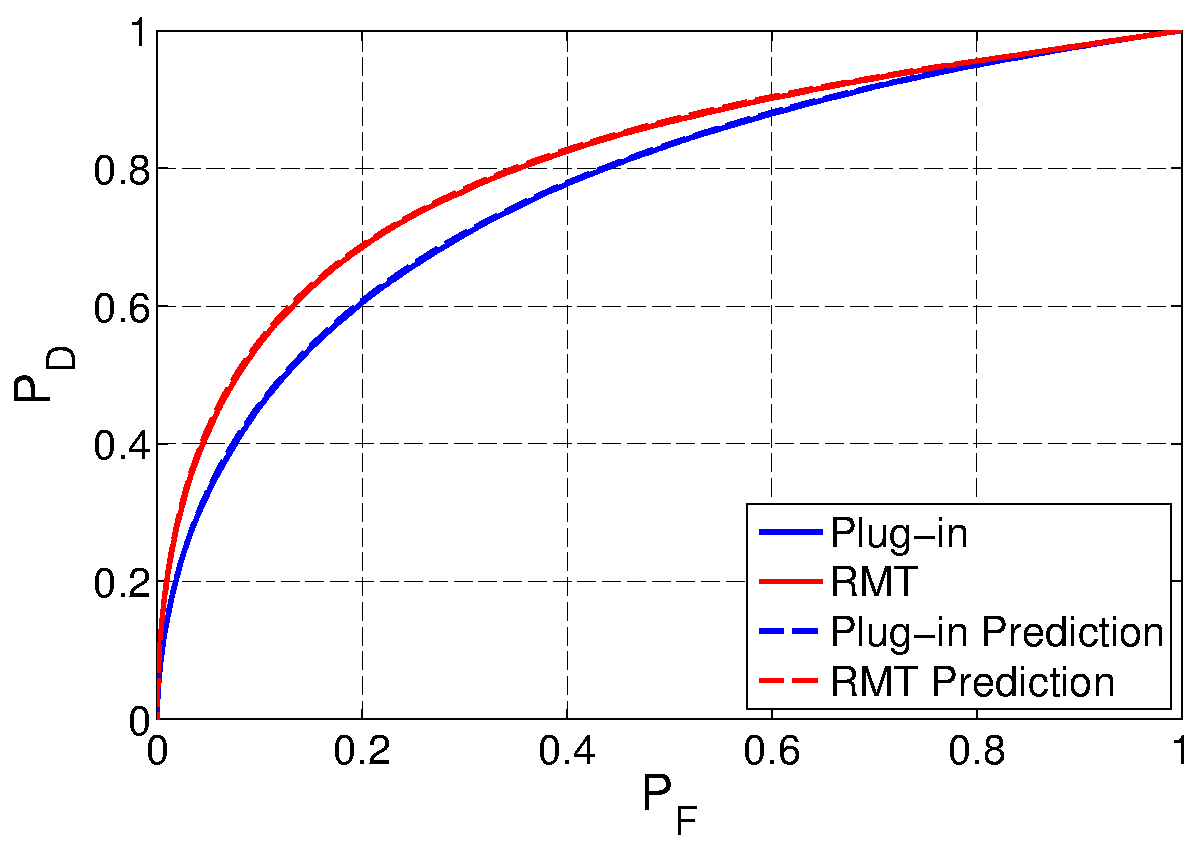
\includegraphics[width=3in]{msd_missing/figures/basic_roc.pdf}
\caption{Empirical and theoretical ROC curves for the plug-in and RMT matched subspace detectors. Empirical ROC curves were simulated with $n=500$, $m=500$, $k=2$, $\Sigma=\diag(3,0.1)$, and $p=0.8$. However, as $\sigma_2$ is below the critical threshold, $k_{\text{eff}} = 1$. The empirical ROC curves were computed using $5000$ test samples and averaged over 25 trials. $x$ was generated randomly for training samples but fixed for test samples. The theoretical ROC curves were obtained using (\ref{eq:roc}). Note the excellent agreement and the performance gain realized by the RMT detector.}\vskip-0.45cm
\label{fig:roc1}
\end{figure}


\subsection{ROC Curves}

We consider a setting where $k_{\text{eff}} = 1 < k = 2$. For this setting, as seen in Figure \ref{fig:roc1}, for any false alarm rate ($P_F$), the RMT detector achieves a higher probability of detection ($P_D$), demonstrating the sub-optimality of the plug-in detector. This is expected because $k_\text{eff}<k$ so that the plug-in detector is employing uninformative subspace components. The theoretical ROC curves in (\ref{eq:roc}) match the empirically generated ROC curves validating the performance predictions of (\ref{eq:roc}) which rely on Theorem \ref{th:angles}.

\subsection{Effect of Missing Data}
Figure \ref{fig:sparsity} examines the performance of each detector as a function of $p$. Again we observe the sub-optimality of the plug-in detector. The theoretical $P_D$ prediction in (\ref{eq:roc}) matches empirically achieved $P_D$ for both detectors. As expected, as $p$ decreases, the achieved probability of detection decreases. We note the presence of a critical $p_{\text{crit.}} : = \sqrt{c}/\max_{i}(\sigma_{i}^{2})$ obtained from Theorem \ref{th:angles}, below which (in the large system limit) we may only achieve $P_D=P_F$; the rounding in Figure \ref{fig:sparsity} is attributed to finite system approximation error.

\begin{figure}[t]
\centering
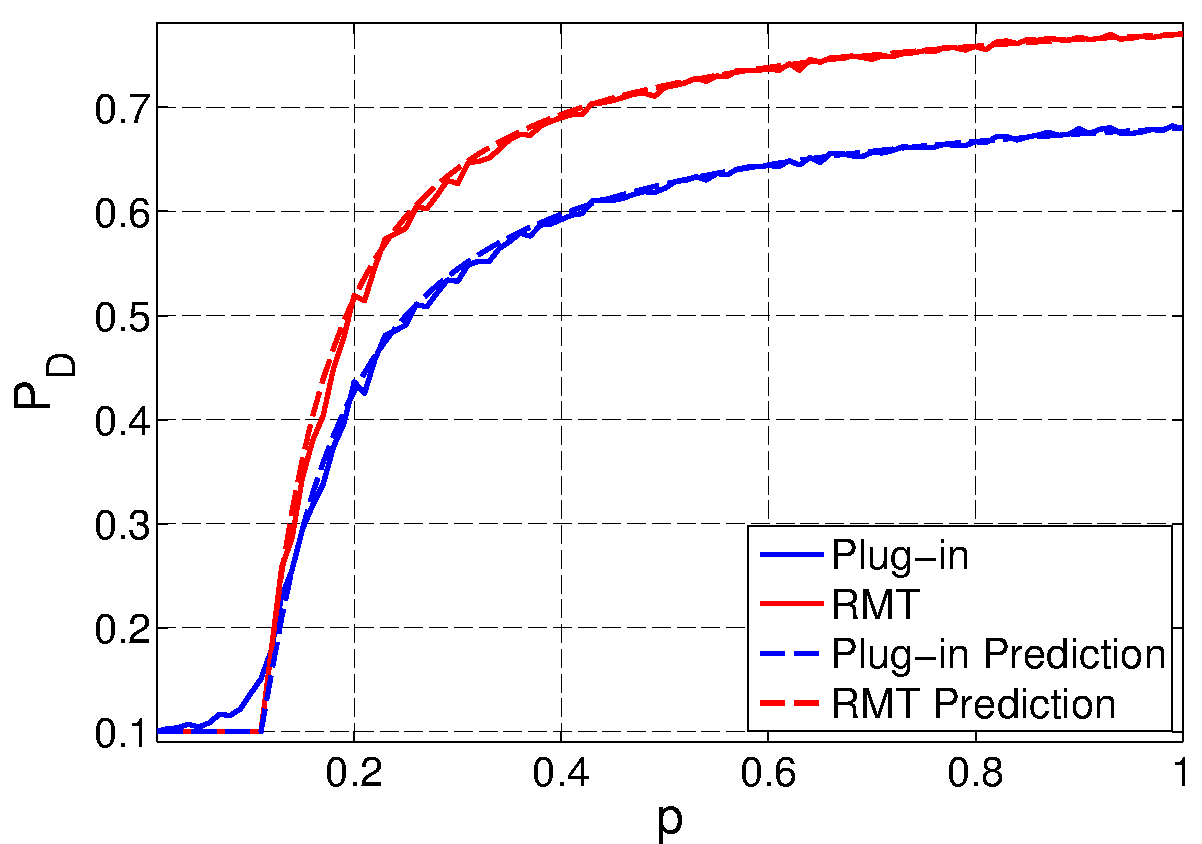
\includegraphics[width=3in]{msd_missing/figures/sparsity.pdf}
\caption{Empirically computed probability of detection, $P_D$, for a fixed probability of false alarm, $P_F=0.1$, for various $p$. Here, $n=1000$, $m=1000$, $k=2$, $\Sigma=\diag(3,0.1)$. $P_D$ was computed using (\ref{eq:roc}) and $x$ was generated as described in Figure \ref{fig:roc1}. For values of $p \leq 1/9$, $k_\text{eff}=0$ and performance degrades to $P_D = P_F +o(1)$ for both detectors. As $p$ increases, $k_\text{eff}=1$ allowing the detectors to achieve better than random guessing performance. When $k_\text{eff}>0$ the plug-in detector is sub-optimal for all values of $p$.}\vskip-0.45cm
\label{fig:sparsity}
\end{figure}



